% VLDB template version of 2020-08-03 enhances the ACM template, version 1.7.0:
% https://www.acm.org/publications/proceedings-template

\documentclass[sigconf, nonacm]{acmart}

%% The following content must be adapted for the final version
\newcommand\vldbdoi{XX.XX/XXX.XX}
\newcommand\vldbpages{XXX-XXX}
\newcommand\vldbvolume{19}
\newcommand\vldbissue{1}
\newcommand\vldbyear{2026}
\newcommand\vldbauthors{\authors}
\newcommand\vldbtitle{\shorttitle}
\newcommand\vldbavailabilityurl{https://github.com/apache/mahout}
% use 'plain' for review, 'empty' for camera ready
\newcommand\vldbpagestyle{plain}

% figure placement
\usepackage{listings}
\usepackage{xcolor}

\lstset{
  language=Python,
  basicstyle=\ttfamily\scriptsize,
  keywordstyle=\color{blue!70!black}\bfseries,
  commentstyle=\color{green!50!black},
  stringstyle=\color{red!60!black},
  frame=single,
  breaklines=true,
  columns=fullflexible,
}

\begin{document}
\title{Apache Mahout QDP: GPU-Accelerated Quantum Data Processing}

\author{Guan-Ming Chiu}
\affiliation{%
  \institution{National Taiwan University}
  \city{Taipei}
  \country{Taiwan}
}
\email{gmchiu@arbor.ee.ntu.edu.tw}

% Add more authors here
% \author{Name}
% \affiliation{%
%   \institution{Institution}
%   \city{City}
%   \country{Country}
% }
% \email{email@example.com}

%%
%% Abstract
%%
\begin{abstract}
Quantum machine learning (QML) pipelines require encoding classical data into quantum states before any computation can proceed.
Existing frameworks such as PennyLane and Qiskit perform this encoding on the CPU, one vector at a time, creating a severe data loading bottleneck that dominates end-to-end training time.
We demonstrate \textbf{QDP} (Quantum Data Processing), a GPU-accelerated data processing engine built with Rust and CUDA as part of Apache Mahout.
QDP provides a complete pipeline from columnar storage formats (Parquet, Arrow) through normalization and quantum state encoding to zero-copy tensor output via DLPack, achieving orders-of-magnitude speedups over existing frameworks.
Our interactive demonstration allows users to (1)~explore the end-to-end encoding pipeline with configurable parameters, (2)~compare latency and throughput against PennyLane and Qiskit in real time, and (3)~analyze performance scaling across qubit counts.
\end{abstract}

\maketitle

%%% do not modify the following VLDB block %%
%%% VLDB block start %%%
\pagestyle{\vldbpagestyle}
\begingroup\small\noindent\raggedright\textbf{PVLDB Reference Format:}\\
\vldbauthors. \vldbtitle. PVLDB, \vldbvolume(\vldbissue): \vldbpages, \vldbyear.\\
\href{https://doi.org/\vldbdoi}{doi:\vldbdoi}
\endgroup
\begingroup
\renewcommand\thefootnote{}\footnote{\noindent
This work is licensed under the Creative Commons BY-NC-ND 4.0 International License. Visit \url{https://creativecommons.org/licenses/by-nc-nd/4.0/} to view a copy of this license. For any use beyond those covered by this license, obtain permission by emailing \href{mailto:info@vldb.org}{info@vldb.org}. Copyright is held by the owner/author(s). Publication rights licensed to the VLDB Endowment. \\
\raggedright Proceedings of the VLDB Endowment, Vol. \vldbvolume, No. \vldbissue\ %
ISSN 2150-8097. \\
\href{https://doi.org/\vldbdoi}{doi:\vldbdoi} \\
}\addtocounter{footnote}{-1}\endgroup
%%% VLDB block end %%%

%%% do not modify the following VLDB block %%
%%% VLDB block start %%%
\ifdefempty{\vldbavailabilityurl}{}{
\vspace{.3cm}
\begingroup\small\noindent\raggedright\textbf{PVLDB Artifact Availability:}\\
The source code, data, and/or other artifacts have been made available at \url{\vldbavailabilityurl}.
\endgroup
}
%%% VLDB block end %%%

%% ============================================================
%% 1. INTRODUCTION
%% ============================================================
\begin{figure}[t]
  \centering
  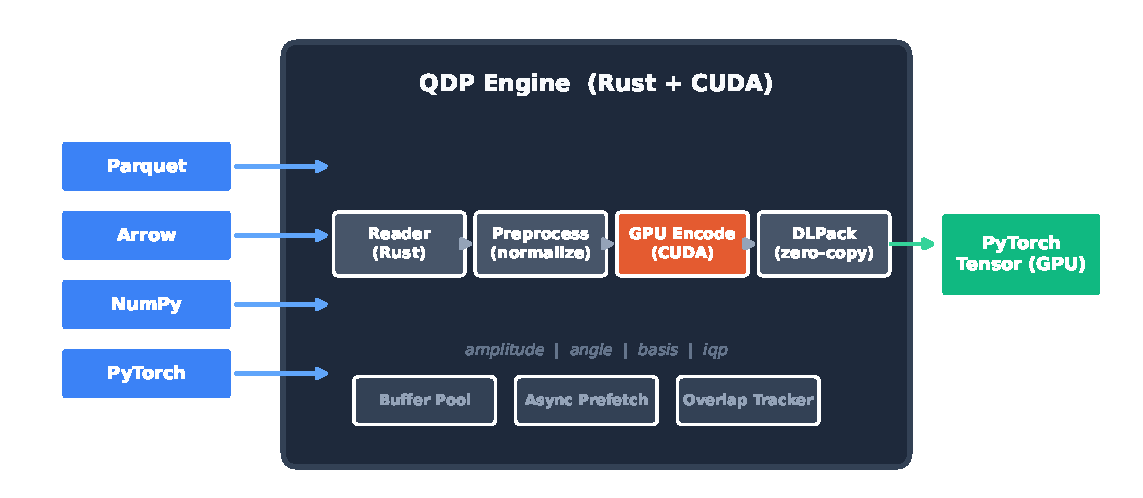
\includegraphics[width=\linewidth]{figures/architecture}
  \caption{QDP pipeline architecture. Classical data flows from columnar storage through Rust-based readers and preprocessing into CUDA-accelerated encoding kernels, producing GPU-resident quantum state tensors via DLPack.}
  \label{fig:architecture}
\end{figure}

\begin{figure*}[t]
  \centering
  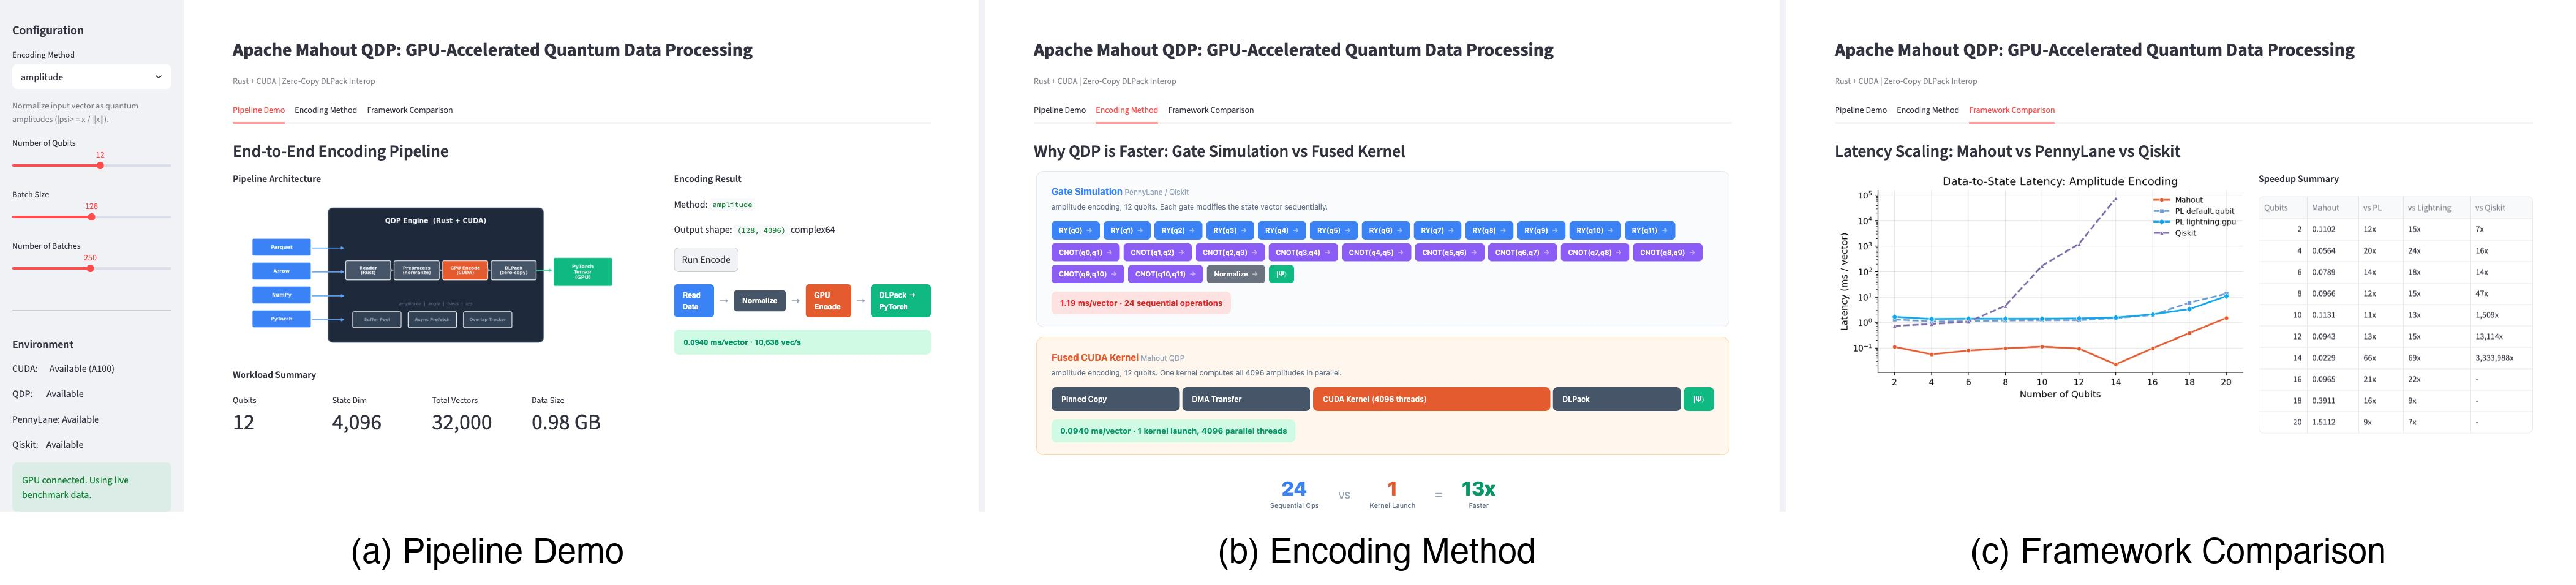
\includegraphics[width=\linewidth,height=4.2cm,keepaspectratio]{figures/demo}
  \vspace{-0.3cm}
  \caption{QDP interactive demonstration. (a)~Pipeline demo with live encoding and animated pipeline stages. (b)~Encoding method comparison: gate simulation (sequential) vs fused CUDA kernel (parallel). (c)~Framework comparison with latency scaling across 2--20 qubits for four frameworks.}
  \label{fig:demo}
\end{figure*}

\section{Introduction}

Quantum machine learning (QML) combines quantum computing with classical machine learning to explore potential computational advantages~\cite{biamonte2017, schuld2021}.
A critical step in every QML pipeline is \emph{quantum data encoding}: transforming classical feature vectors into quantum states that can be processed by parameterized quantum circuits.
Common encoding strategies include amplitude encoding, angle encoding, basis encoding, and IQP-style encoding~\cite{schuld2021}.

In current practice, frameworks such as PennyLane~\cite{pennylane} and Qiskit~\cite{qiskit} implement encoding by constructing and simulating a quantum circuit for each input vector.
Even with GPU-accelerated backends (e.g., Lightning.GPU, Aer GPU), the encoding step remains sequential and per-vector, creating a bottleneck that grows with qubit count.
For a 16-qubit system, each state vector has $2^{16} = 65{,}536$ complex amplitudes; encoding thousands of training samples at this scale can take minutes with existing tools, while the subsequent quantum circuit simulation on GPU completes in seconds.
This \emph{data starvation} problem, where the GPU sits idle waiting for encoded data, is analogous to the classical ML data loading bottleneck that motivated systems like PyTorch DataLoader~\cite{pytorch}, but has received almost no attention in the quantum computing community.

We present \textbf{QDP} (Quantum Data Processing), a GPU-accelerated quantum data encoding engine that is part of Apache Mahout.
QDP addresses the data loading bottleneck with three key design decisions:
\begin{enumerate}
\item \textbf{Rust + CUDA core.} The entire pipeline, from file I/O through encoding to GPU memory placement, is implemented in Rust with custom CUDA kernels, eliminating Python overhead and GIL contention.
\item \textbf{Columnar format integration.} QDP reads directly from Parquet~\cite{parquet} and Arrow IPC~\cite{arrow} files using native Rust readers, avoiding redundant serialization and deserialization.
\item \textbf{Zero-copy output.} Encoded quantum states are exposed to Python via DLPack~\cite{dlpack}, enabling zero-copy transfer to PyTorch tensors on GPU without any data movement.
\end{enumerate}

Together, these design choices yield \textbf{up to 1{,}000$\times$} speedup in data-to-state latency compared to PennyLane and Qiskit, as we demonstrate in our interactive system.

%% ============================================================
%% 2. SYSTEM OVERVIEW
%% ============================================================
\section{System Overview}

\autoref{fig:architecture} shows the QDP pipeline architecture.
The system consists of four stages connected by an asynchronous buffer pool.

\textbf{Reader.}
The reader stage ingests data from multiple formats: Apache Parquet, Arrow IPC, NumPy \texttt{.npy}, PyTorch \texttt{.pt}, and TensorFlow TFRecord.
For Parquet and Arrow, QDP uses native Rust implementations (via the \texttt{arrow-rs} and \texttt{parquet} crates) that decode columnar data directly into contiguous memory buffers, avoiding Python-based deserialization.
A \emph{streaming} mode for Parquet reads row groups incrementally, enabling processing of datasets larger than available memory.
QDP also supports remote object storage URLs (\texttt{s3://}, \texttt{gs://}) via the \texttt{object\_store} crate, allowing direct ingestion from cloud data lakes without intermediate downloads.

\textbf{Preprocessing.}
Raw feature vectors are normalized according to the requirements of each encoding method.
For amplitude encoding, this involves L2 normalization to ensure $\sum_i |a_i|^2 = 1$.
Preprocessing runs on the CPU using multi-threaded Rust code and writes results into pinned host memory for efficient DMA transfer to the GPU.

\textbf{GPU Encoding.}
Existing frameworks implement encoding by simulating a quantum circuit through sequential gate applications to a state vector.
QDP instead provides fused CUDA kernels that directly compute the encoded state vector from classical input data, bypassing circuit simulation entirely and supporting native batching across multiple samples in one kernel launch.
QDP supports four methods: \emph{amplitude} (normalize as quantum amplitudes), \emph{angle} (map features to rotation angles), \emph{basis} (encode integer as $|k\rangle$), and \emph{IQP} (entangling interactions between qubits).

\textbf{Zero-Copy Output.}
Encoded complex-valued state vectors remain in GPU memory and are wrapped in a DLPack capsule~\cite{dlpack}.
Python consumers call \texttt{torch.from\_dlpack()} to obtain a PyTorch tensor backed by the same GPU allocation, with no host-device copy or memory duplication.
Ownership is managed through DLPack's reference-counted deleter protocol, ensuring the GPU buffer is freed only after all consumers release it.

\subsection{Pipeline Infrastructure}

Three subsystems maximize GPU utilization:

\textbf{Dual-stream pipeline.}
QDP allocates two CUDA streams: one for host-to-device memory copies and one for compute kernels.
A CUDA event synchronizes the streams: the copy stream signals completion via \texttt{cudaEventRecord}, and the compute stream waits via \texttt{cudaStreamWaitEvent} before launching the encoding kernel.
This double-buffered design ensures that batch $i{+}1$ is being transferred while batch $i$ is being encoded, hiding transfer latency behind compute.

\textbf{Pinned buffer pool.}
Repeated \texttt{cudaHostAlloc}/\texttt{cudaFreeHost} calls are expensive.
QDP pre-allocates a fixed pool of page-locked host buffers at initialization.
Buffers are checked out via RAII handles and automatically returned on drop, amortizing allocation cost across all batches.
A condition variable blocks producers when all buffers are in use, providing natural backpressure.

\textbf{Overlap tracker.}
An instrumentation layer records timestamps for copy and compute events on each batch, computing the fraction of time that both streams are active simultaneously.
This metric, exposed through the Python API, helps users identify whether their workload is transfer-bound or compute-bound and tune batch sizes accordingly.

\subsection{Programming Interface}

QDP exposes two Python APIs. The \textbf{one-shot API} encodes an entire file into a single GPU tensor, suitable for small datasets that fit in memory:

\begin{lstlisting}
import qumat.qdp as qdp
engine = qdp.QdpEngine(device_id=0)
qt = engine.encode("data.parquet", num_qubits=16,
                   encoding_method="amplitude")
tensor = torch.from_dlpack(qt)  # (N, 65536) complex64
\end{lstlisting}

\noindent The \textbf{iterator API} provides DataLoader-style batching with a builder pattern, streaming encoded batches for large-scale training loops:

\begin{lstlisting}
loader = (qdp.QuantumDataLoader(device_id=0)
          .qubits(16).encoding("amplitude")
          .batches(100, size=64)
          .source_file("data.parquet"))
for batch in loader:
    state = torch.from_dlpack(batch)  # (64, 65536)
\end{lstlisting}

\noindent The iterator internally drives the dual-stream pipeline (\S2.1), releasing the Python GIL during Rust/CUDA execution so that model training can proceed concurrently.
Input sources include local files (Parquet, Arrow, NumPy, PyTorch, TFRecord), in-memory Python lists, NumPy arrays, PyTorch tensors, and remote URLs (\texttt{s3://}, \texttt{gs://}).
A \texttt{QdpBenchmark} builder provides one-call throughput and latency measurement without requiring manual timing code.

%% ============================================================
%% 3. DEMONSTRATION OVERVIEW
%% ============================================================
\section{Demonstration}

We provide an interactive web-based demonstration built with Streamlit that showcases QDP's capabilities through three scenarios.
The demonstration runs on a machine equipped with an NVIDIA GPU and allows attendees to interact with the system in real time.

\subsection{Scenario 1: Pipeline Demo}

In the first scenario (\autoref{fig:demo}a), attendees explore the end-to-end encoding pipeline.
A sidebar provides global configuration: encoding method (amplitude, angle, basis, IQP), qubit count (2--20), batch size (1--256), and number of batches (10--500).
The main panel displays the pipeline architecture diagram alongside a workload summary showing the state vector dimension ($2^n$), total number of vectors, and estimated data size in GB.
Clicking ``Run Encode'' triggers a real-time encoding pass through the QDP engine.
An animated pipeline visualization appears below the button, sequentially highlighting each stage (Read Data, Normalize, GPU Encode, DLPack) to illustrate the data flow.
The measured per-vector latency and aggregate throughput are displayed upon completion.
Attendees can freely adjust parameters and re-run, observing how encoding cost changes with qubit count, encoding method, and batch configuration.

\subsection{Scenario 2: Encoding Method}

The second scenario (\autoref{fig:demo}b) visually explains \emph{why} QDP is faster than existing frameworks.
Two side-by-side cards contrast the gate simulation approach used by PennyLane and Qiskit with QDP's fused CUDA kernel.
The upper card (Gate Simulation) displays each quantum gate as a colored pill: RY gates for rotation, CNOT gates for entanglement, and a final normalization step.
Gates appear sequentially via CSS animation, emphasizing the per-gate overhead.
The lower card (Fused CUDA Kernel) shows QDP's four-stage pipeline (pinned copy, DMA transfer, CUDA kernel, DLPack), where a single kernel launch computes all $2^n$ amplitudes in parallel.
A summary bar at the bottom highlights the contrast: for 12-qubit amplitude encoding, gate simulation requires 24 sequential operations while QDP uses a single kernel launch, achieving 13$\times$ speedup.
Changing the qubit count or encoding method in the sidebar dynamically updates the gate list, operation count, and speedup ratio, allowing attendees to explore how circuit complexity grows with qubit count.

\subsection{Scenario 3: Framework Comparison}

The third scenario (\autoref{fig:demo}c) presents quantitative performance data across Mahout QDP, PennyLane (both CPU and GPU backends), and Qiskit.
A latency scaling chart plots per-vector encoding time on a log scale across 2--20 qubits, with a speedup table alongside.
Switching the encoding method in the sidebar instantly updates both views.
QDP's advantage is consistent across all methods and grows with qubit count, reaching up to 1{,}000$\times$ over PennyLane for angle encoding at 20 qubits.

%% ============================================================
%% 4. PRELIMINARY EVALUATION
%% ============================================================
\section{Evaluation}

We evaluate QDP on an NVIDIA A100 GPU (80\,GB) with amplitude, angle, and basis encoding across 2--20 qubits.
We compare against PennyLane \texttt{default.qubit}, PennyLane \texttt{lightning.gpu} (CUDA-accelerated), and Qiskit (\texttt{initialize()} for amplitude, \texttt{RY}/\texttt{X} gates for angle/basis via \texttt{Statevector.from\_instruction}).
All measurements include GPU transfer time.

\textbf{Scaling.}
\autoref{fig:eval} shows latency scaling across qubit counts for all three encoding methods, comparing four frameworks.
QDP consistently achieves the lowest latency across all configurations, even against PennyLane's GPU-accelerated \texttt{lightning.gpu} backend.
For angle encoding at 20 qubits, QDP (0.27\,ms) is 1{,}018$\times$ faster than PennyLane \texttt{default.qubit} (274\,ms) and 24$\times$ faster than \texttt{lightning.gpu} (6.5\,ms).
For basis encoding, the gap is similarly large: QDP (0.26\,ms) vs Qiskit (180\,ms) at 20 qubits.
Qiskit's circuit-based amplitude encoding (\texttt{initialize()}) grows exponentially, reaching 171\,ms at just 10 qubits, while QDP remains at 0.11\,ms.
The advantage stems from QDP's fused kernel approach: where PennyLane and Qiskit apply $O(n)$ to $O(n^2)$ sequential gate operations, QDP computes all $2^n$ amplitudes in a single parallel kernel launch.

\begin{figure}[t]
  \centering
  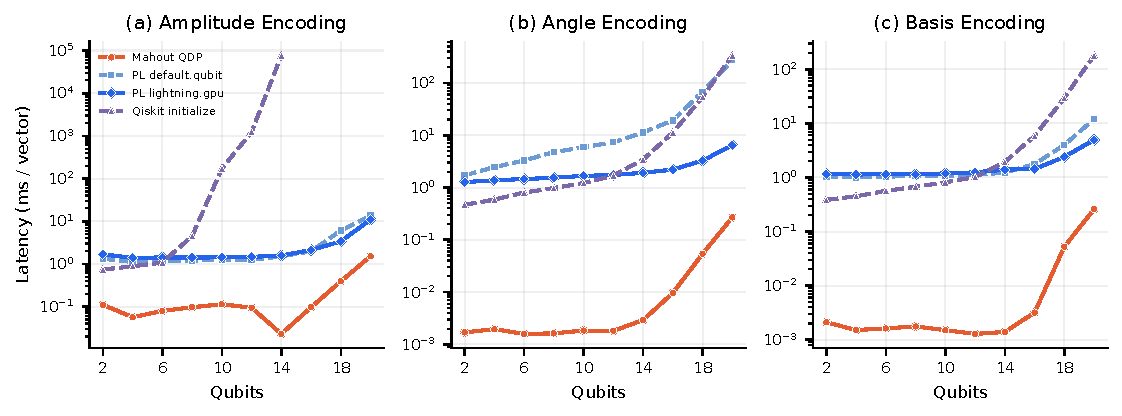
\includegraphics[width=\linewidth]{figures/eval_scaling}
  \caption{Data-to-state latency scaling (ms/vector, log scale) for amplitude, angle, and basis encoding across four frameworks. QDP (orange) achieves orders-of-magnitude lower latency than both CPU and GPU backends of existing frameworks.}
  \label{fig:eval}
\end{figure}

\textbf{Correctness.}
Since QDP bypasses circuit simulation with fused CUDA kernels, correctness validation is essential.
We compare QDP's encoded states against Qiskit across all three encoding methods (amplitude, angle, basis) and 10 qubit counts from 2 to 20, using float64 precision with 50 random input vectors per configuration.
\autoref{tab:correct} shows the maximum amplitude difference is below $10^{-16}$ (machine epsilon) in every case, confirming that QDP produces numerically identical quantum states despite using a fundamentally different computation path.

\begin{table}[h]
  \caption{Max amplitude difference: QDP vs Qiskit (float64).}
  \label{tab:correct}
  \begin{tabular}{lrrr}
    \toprule
    Qubits & Amplitude & Angle & Basis \\
    \midrule
    4  & $1.1 \times 10^{-16}$ & $2.2 \times 10^{-16}$ & $0$ \\
    8  & $5.6 \times 10^{-17}$ & $2.8 \times 10^{-16}$ & $0$ \\
    12 & $1.4 \times 10^{-17}$ & $8.3 \times 10^{-17}$ & $0$ \\
    16 & $6.9 \times 10^{-18}$ & $4.2 \times 10^{-17}$ & $0$ \\
    20 & $1.7 \times 10^{-18}$ & $1.7 \times 10^{-17}$ & $0$ \\
    \bottomrule
  \end{tabular}
\end{table}

\textbf{Case study: SVHN classification.}
To validate end-to-end impact, we train an IQP-based variational quantum classifier on the SVHN dataset~\cite{svhn} (binary classification: digits 1 vs 7, 200 samples, 200 training iterations) across 4--10 qubits.
We compare four configurations: QDP and PennyLane, each with CPU and GPU training backends.
QDP performs one-shot encoding ($\sim$10\,ms total for all samples regardless of qubit count), while PennyLane re-encodes via IQP gates on every forward pass.
All four configurations converge to identical test accuracy (0.675), confirming that QDP's fused kernel is functionally equivalent to PennyLane's gate-by-gate simulation in downstream QML tasks.
\autoref{tab:e2e} shows QDP-GPU achieves up to 1.51$\times$ training speedup over PennyLane \texttt{lightning.gpu}.
The speedup grows with qubit count because IQP circuits have $O(n^2)$ parametric gates; at 10 qubits, QDP eliminates 55 gate operations per forward pass.

\begin{table}[h]
  \caption{End-to-end training time (seconds) on SVHN IQP classification. All configs achieve identical accuracy (0.675).}
  \label{tab:e2e}
  \begin{tabular}{rrrrr}
    \toprule
    Qubits & PL-GPU & QDP-GPU & Speedup \\
    \midrule
    4  & 44.8 & 36.4 & 1.23$\times$ \\
    6  & 65.2 & 43.2 & 1.51$\times$ \\
    8  & 80.7 & 59.4 & 1.36$\times$ \\
    10 & 100.1 & 71.1 & 1.41$\times$ \\
    \bottomrule
  \end{tabular}
\end{table}

%% ============================================================
%% 5. RELATED WORK
%% ============================================================
\section{Related Work}

\textbf{Quantum data encoding.}
Schuld and Petruccione~\cite{schuld2021} provide a comprehensive survey of encoding strategies for QML.
Amplitude encoding is the most commonly used method for variational classifiers, as it can represent $2^n$ features with $n$ qubits, but requires $O(2^n)$ operations for state preparation.
Angle and basis encodings trade expressiveness for simpler circuit constructions~\cite{biamonte2017}.
Preskill~\cite{preskill2018} discusses the challenges of the NISQ era, where limited qubit counts and noise make efficient classical preprocessing even more critical for practical QML workloads.

\textbf{Quantum software frameworks.}
PennyLane~\cite{pennylane} provides automatic differentiation for hybrid quantum-classical programs and supports multiple backend simulators.
Qiskit~\cite{qiskit} offers a comprehensive toolchain for circuit construction, transpilation, and execution on IBM hardware.
Both treat data encoding as a preprocessing step without GPU acceleration, constructing states one vector at a time on the CPU.
Neither framework batches encoding or leverages GPU parallelism for state preparation.
QuClassi~\cite{quclassi} demonstrated hybrid quantum-classical architectures at MLSys but did not address the data loading bottleneck.
Q2O~\cite{q2o} applied quantum optimization to database query planning at VLDB 2025, demonstrating growing interest in quantum-data systems in the database community.

\textbf{Classical data loading systems.}
The data starvation problem is well-studied in classical ML: PyTorch DataLoader~\cite{pytorch} introduced multi-process prefetching and pinned memory transfers, NVIDIA DALI provides GPU-accelerated image decoding, and tf.data pipelines overlap I/O with computation.
QDP brings analogous design principles to the quantum data encoding domain, including asynchronous prefetching, pinned buffer pooling, dual-stream pipelining, and zero-copy tensor output.
While these techniques are mature in the classical ML ecosystem, to our knowledge QDP is the first system to apply them to quantum state encoding.

%% ============================================================
%% 6. CONCLUSION
%% ============================================================
\section{Conclusion}

We demonstrated QDP, a GPU-accelerated quantum data processing engine that addresses the data loading bottleneck in QML pipelines.
By implementing the full path from columnar storage to GPU-resident quantum states in Rust and CUDA, QDP achieves up to 1{,}000$\times$ lower latency than PennyLane and Qiskit, and 24$\times$ speedup over PennyLane's GPU-accelerated \texttt{lightning.gpu} backend at 20 qubits.
Key engineering contributions include dual-stream pipelining for overlapping host-to-device transfers with GPU encoding, a pinned buffer pool with RAII-based lifecycle management, and zero-copy DLPack interop with PyTorch.

QDP is open source as part of Apache Mahout and supports cloud-native workflows through streaming Parquet ingestion from S3 and GCS.
Future directions include:
(1)~multi-GPU encoding with NCCL-based distribution;
(2)~AMD ROCm/HIP backend for vendor-neutral acceleration;
(3)~broader cloud data lake support (Azure Blob, MinIO, Delta Lake/Iceberg);
(4)~parameterized circuit encoding; and
(5)~integration with quantum hardware backends for NISQ devices.

%% ============================================================
%% ACKNOWLEDGMENTS & REFERENCES
%% ============================================================

\begin{acks}
The authors initiated the QDP project within Apache Mahout and serve as PMC members and committers.
We thank Chia-Ping Tsai, Andrew Musselman, and Trevor Grant for their mentorship and guidance on the Apache Mahout project.
We also thank the Mahout community and the Apache Taipei\footnote{\url{https://github.com/opensource4you}} community for their support.
\end{acks}

\bibliographystyle{ACM-Reference-Format}
\bibliography{references}

\end{document}
\endinput
